\section{Ideas}
This section contains things that have been discussed but not which are still unclear. 
It will need to be deleted at some point.

\subsection{Minimising insertion cost}
Yngvi has an interesting idea; before insertion, calculate all possible paths between the start cluster and goal cluster. 
In our case, we can use dominance to immediately prune some of these paths. 
This then limits the number of edges that must be inserted into the abstract graph to connect the start and goal (we only connect to entrances that appear on a hierarchical path.
It's quite a nice technique; one easily applied to any hierarchical planner (HPA*, HAA* etc).

\subsection{Greedy path refinement}
In order to refine a hierarchical path we can use a 1-step lookahead to create a series of incrementally refined subplans which minimise costs between all entrances that must be traversed.
This requires caching a set of endpoint pairs for each edge in the abstract graph, each representing the endpoints of a path between the two entrances of cost lowerbound (note that there may be several such paths).
Consider as an example the hierarchical path $\Pi_{H} = \lbrace n_{1}, n_{2}, n_{3}, n_{4} \rbrace$ where each element is an abstract node that represent an entrance to be traversed.
In particular, $n_{1}$ is an entrance in the start cluster, $n_{4}$ is an entrance in the goal cluster and $n_{2}, n_{3}$ are intermediaries. 
The refinement process involves several steps:
\begin{itemize}
\item{To insert the start position into the abstract graph we begin by using a lookhead to identify which nodes in $n_{1}$  and $n_{2}$ minimise distance between the two entrances (call these endpoints $w \in n_{1}$ and $x \in n_{2}$). 
Note that this operation may return a set of nodes if multiple paths of minimum length exist.
Once identified, the start position is then connected to each such node in $n_{1}$.}
\item{Again using a lookahead, we identify which nodes in $n_{2}$ and $n_{3}$ minimise distance between the two entrances (call these endpoints $y \in n_{2}$ and $z \in n_{3}$);}
\item{It remains to calculate the cost of the minimum length path between $x$ and $y$; we can use the manhattan heuristic for this which perfectly estimates the distance between two nodes in an entrance.}
\item{Proceed in this way to incrementally extract the costs of subpaths on the optimal path all the way to the entrance to the goal cluster.} 
\item{Connect the goal to the transition point in $n_{4}$ that minimise distance to $n_{3}$ and use the manhattan heuristic to compute the length of the path between this node and the transition point in the previous step. }
\end{itemize}
In some situations (such as on an empty map) there may be several transition points from the start/goal cluster that minimise distance to the next entrance on the hierarchical path. 
In this case, we connect to all such transition points and refine up to $n \times m$ paths where $n$ and $m$ are the number of such transition points in the entrance to the start and goal cluster respectively.

\begin{figure}[htbp]
	\vspace{-9pt}
	\caption{\emph{Refinement example} Dashed lines represent optimal length edges whose costs are not known apriori.}
       \begin{center}
          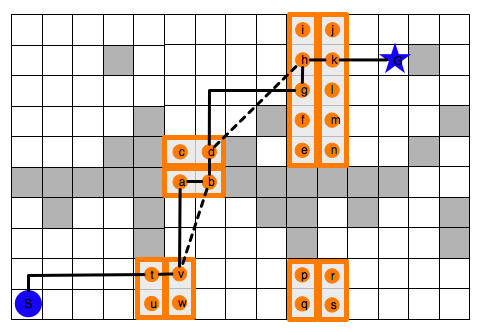
\includegraphics[scale=0.35, trim = 20mm 9mm 20mm 0mm]{diagrams/refinementexample.png}
       \end{center}
       \label{ia-fig:refinement}
	\vspace{-6pt}
\end{figure}

\subsection{Better heuristics}
We can use intervals to compute better heuristics to guide a low-level search.
$h(n) = g(nextentrance, goal) + manhattan(n, nextentrance)$

\subsection{Other Ideas}

The following two ideas assume that we need to perform a refinment search
inside a corridor.
A corridor of an abstract path is the union of all corridors between
consecutive abstract nodes along the abstract path.
Corridors between two abstract nodes (i.e., entrances $E_1$ and $E_2$)
that belong to the same cluster are precomputed.
For the $i$-th tile of $E_1$ and the $j$-th tile of $E_2$,
we compute one shortest path $\pi(i,j)$ between the two tiles.
The union of such paths for all combinations $(i,j)$
compose the corridor.

\paragraph{Minimizing corridor size.}
We should actively try to minimize the number of the tiles in the corridor.
In this way, we may have a much smaller space to explore in a refinement search.
Obtaining a corridor of miminal size might be computationally challenging,
but good approximations could be obtained with a greedy approach.
E.g., \emph{process} pairs $(i,j)$ in increasing order according to the length of $\pi(i,j)$.
Processing a pair $(i,j)$ means to select a shortest path $\pi(i,j)$ and
add its tiles to the corridor.
If several optimal paths exist for a pair of tiles $(i,j)$ at hand,
pick the one that has the most in common with the existing part
of the corridor built so far.

\paragraph{Pruning nodes in the first part of the corridor.}
Assume we have an entrance with $k$ tiles
along an abstract path currently being refined.
As soon as all $k$ tiles have been expanded in a refinement search, there is no need
to expand nodes that are physically before this entrance in the corridor.
Optimality is preserved.

\paragraph{Discussion.}
We call a regular A* search (inside the corridor), enhanced with the two ideas
presented earlier an \emph{enhanced refinement search}.
Enhanced refinement search could handle some of the problem properties
mentioned in previous meetings quite efficiently.
For example, consider a property pointed out by Daniel:
For a given pair of entrances $E_1$ and $E_2$, assume there is only
one pair of tiles $(i_0, j_0)$ that minimizes the path length
between any tiles on the two entrances.
If only straight moves are considered, then
the path from the $i_0$-th tile of $E_1$
to the $j_0$-th tile of $E_2$
(with these two ends included) is guaranteed
to belong to at least one optimal solution.
As a result, the search can be decomposed (with no optimality loss) as
a search from start to $i_0$ + a search from $i_0$ to $j_0$ (trivial) + a search from $j_0$ to target.

Enhanced refinement search would perform a similar problem decomposition,
as shown here.
Firstly,
by trying to minimize the size of the corridor we end up with a one-width tunnel,
namely the path between $i_0$ and $j_0$.
Secondly, as soon as we expand $i_0$, 
we don't expand nodes that are physically placed before $i_0$ in the corridor.
This is equivalent to searching first to achieve $i_0$, 
then going to $j_0$ along the corridor,
and then searching
from $j_0$ towards the target.

Note that enhanced refinement search handles more general cases as well
(though we know little about the performance unless we run experiments).
E.g., it works even if diagonal moves are allowed or
no one-width corridors can be built.

